\documentclass{article}
\usepackage[T1]{fontenc}
\usepackage{lmodern}
\usepackage{graphicx}
\usepackage{amsmath,amssymb}
\usepackage[a4paper,margin=2cm]{geometry}
\usepackage[absolute,overlay]{textpos}
\setlength{\TPHorizModule}{1mm}
\setlength{\TPVertModule}{1mm}
\usepackage[indonesian]{babel}
\usepackage{hyperref}
\setlength{\emergencystretch}{2em}
% unit: Halaman 39

\begin{document}

% === Halaman 39 (python/native) ===

•

Dengan karakteristik seperti terebut, maka distribusi kemunculan 

huruf di dalam cipherteks relatif mendekati seragam (uniform) dan 

histogramnya cenderung flat (datar)

•

Histogram yang flat akan menyulitkan kriptanalisis memecahkan 

cipherteks dengan metode analisis frekuensi

39

Flat histogram

Bukan flat histogram

A  B C  D ………….…………………………………..……X  Y   Z

A  B C  D …………………………………………X  Y   Z

% deskripsi: gambar native xref 168
\noindent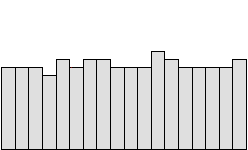
\includegraphics[width=0.85\textwidth]{../../images/python/page_039_img_01.png}

% deskripsi: gambar native xref 171
\noindent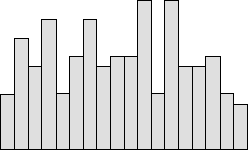
\includegraphics[width=0.85\textwidth]{../../images/python/page_039_img_02.png}

\end{document}
